\documentclass{scrartcl}
\usepackage[a4paper, total={7in, 10in}]{geometry}
\usepackage{stmaryrd}
\usepackage{amsthm}
\usepackage{amssymb}
\usepackage{amsmath}
\usepackage{algorithm2e}
\usepackage{hyperref}
\usepackage{comment}
\usepackage[french]{babel}
\usepackage{color}
\usepackage{tikz}
\usepackage{graphicx}
\usetikzlibrary{automata, arrows.meta, positioning}
\usepackage{MacrosArt}

%% Generated by ipescript page-labels figs.pdf
%% Do not edit
\newcommand{\ipeFigexcarte}{1}
\newcommand{\ipeFigKKnIpqcompl}{2}
\newcommand{\ipeFigcartetrivperf}{3}
\newcommand{\ipeFigextrivperf}{4}
\newcommand{\ipeFigIpqIrsMap}{5}
\newcommand{\ipeFigIpqIrsItuMap}{6}
\newcommand{\ipeFigtemoinK}{7}
\newcommand{\ipeFigpointabuse}{8}
\newcommand{\ipeFigcographsepind}{9}
\newcommand{\ipeFigfirsttemoin}{10}
\newcommand{\ipeFigfirsttemoinquatriparti}{11}
\newcommand{\ipeFigsecondtemoinquatriparti}{12}

\begin{document}

\title{Stage Map Graphs}

\author{José Lorgeré}

\maketitle

\begin{flushleft}

\tableofcontents

\section*{Introduction}

La notion de planarité est une des notions les plus influentes de la théorie des graphes, ayant motivé le célèbre théorème des $4$ couleurs,
et l'étude des liens et apports mutuels entre graphes et surfaces topologiques \cite{face2conn}. En $1998$, Chen, Grigni et Papdimitriou
introduisent une notion proche de la planarité, et une nouvelle classe de graphe, les graphes de carte \cite{IntroMap}. Ces derniers
sont définis comme graphes d'intersection de régions d'intérieurs disjoints sur la sphère : les sommets du graphe sont les régions,
si deux régions se touchent, il y a une arrête entre ces dernières. Cette notion peut faire penser à la formulation originale la plus
connue du théorème des $4$ couleurs qui énonce que l'on peut colorier toute carte en $4$ couleurs sans que deux régions voisines
n'aient la même couleur. Les graphes planaires sont en fait tous des graphes de carte. Toutefois, la classe des graphes de carte
est bien plus large que celle des graphes planaires, contenant par exemple des cliques de toutes tailles. Cette dernière a des
propriétés structurelles intéressantes, par exemple, son nombre de cliques maximales étant linéaire en le nombre de ses sommets
\cite{IntroMap}, et l'on peut borner la taille de ses cliques maximales par $\frac{3k}{2}$ où $k$ est le nombre maximal de régions
autorisées à se rencontrer en un point \cite{IntroMap}. Cette classe a également des propriétés algorithmiques intéressantes :
le problème de l'indépendant maximum admet un schéma d'approximation en temps polynômial et le nombre chromatique
peut être $2$-approché en temps polynômial \cite{approxMap}.
\\~\\
Dans leur articule introductif, Chen et al. posent la question de la reconnaissance de cette nouvelle classe de graphe : décider si un
graphe donné est de carte ou non. Il montrent que ce problème est dans NP, et donnent un algorithme polynômial dans un cas particulier,
lorsque les régions recouvrent la sphère et qu'en tout point au plus $4$ régions se rencontrent. En $1998$, Thorup annonce avoir un algorithme
polynômial résolvant le problème \cite{Thorup}. Toutefois, l'algorithme a une complexité estimée de $O(n^{120})$ \cite{n120} et les détails ne
sont jamais publiés. Plus récemment, un algorithme FPT a été obtenu \cite{FptMap} ou le paramètre est la largeur arborescente du graphe.
\\~\\
J'ai travaillé pendant ce stage à l'élaboration d'algorithmes de reconaissances des graphes de carte, et à trouver des caractérisations
combinatoires de ces derniers : après avoir trouvé quelques graphes contre exemple relativement simples, j'ai pu classifier les graphes
de carte trivialement parfaits et les cographes de carte. Certaines de mes réflexions concernant les graphes $3$-connexes de carte, en vue
d'un algorithme généralisant les méthodes utilisées, sont également présentées. Certaines de mes contributions apportant peu au rapport,
par exemple certaines démonstrations parfois longues, sont reléguées en annexe.

\section{Généralités sur les graphes de carte}

\subsection{Résultats et définitions préliminaires}

On commence par définir plus formellement ce que l'on entend lorsque l'on parle de régions et donc de graphes de carte.

\begin{def*}[Carte]
    Une carte est une fonction $f : V \rightarrow \mathcal{P}(\mathbb{S}^2)$ telle que pour tout $v \in V$, $f(v)$
    est homéomorphe à $\mathbb{D}^2$ et telle que pour $v \neq u$, $f(u)$ et $f(v)$ sont d'intérieur disjoints. Si
    $f$ forme un recouvrement de $\mathbb{S}^2$, on la dira sans trou, ou complète. On appelera les $f(v)$ régions
\end{def*}

\begin{def*}[Graphe de carte \cite{IntroMap}]
    Un graphe $G = (V, E)$ est de carte s'il existe une carte $f$ sur $V$ telle que $xy \in E$ si et seulement si
    $f(x) \cap f(y) \neq \varnothing$
\end{def*}

\begin{figure}[h]
    \caption{Un graphe, une carte, et un témoin associés à ce dernier}

    \begin{center}
    \begin{tikzpicture}[auto]
        \begin{scope}[every node/.style={circle, draw}]
            
        \node (a) {$a$};
        \node (h) [left = of a] {$h$};
        \node (e) [right = of a] {$e$};
        \node (b) [below = of h] {$b$};
        \node (g) [below = of b] {$g$};
        \node (c) [right = of g] {$c$};
        \node (d) [below = of e] {$d$};
        \node (f) [below = of d] {$f$};
        \end{scope}

        \path
        (a) edge (b) edge (c) edge (d) edge (e) edge (h)
        (b) edge (c) edge (d) edge (h) edge (g)
        (c) edge (d) edge (g) edge (f)
        (d) edge (e) edge (f);
    \end{tikzpicture}
    \hspace*{1.5cm}
    \includegraphics[page=\ipeFigexcarte, scale = 0.5]{figs}
    \hspace*{1cm}
    \includegraphics*[page=\ipeFigfirsttemoin, scale = 0.38]{figs}
    \end{center}
\end{figure}

La caractérisation suivante permet d'envisager les graphes de carte de manière bien plus combinatoire que la définition précédente.
Si $G$ est un graphe et $S \subset V$, $G[S]$ désigne le sous graphe induit de $G$ par $S$.

\begin{theorem}[Témoins des graphes de carte \cite{IntroMap}]\label{carCarte}
    Un graphe $G = (V, E)$ est de carte si et seulement si il existe $H$ un graphe biparti planaire, de bipartition $V, U$,
    tel que $H^2[V] = G$. Un tel graphe $H$ est appelé graphe témoin de $G$
\end{theorem}

Le témoin est construit depuis une carte comme suit : les sommets de $V$ sont placés à l'intérieur de leur région respective.
Les sommets de $U$ quand à eux représentent les points de rencontre entre différentes régions : si deux régions se rencontrent, on place
un sommet de $U$ dans leur frontière commune et on relie les sommets de $V$ respectifs à ce sommet par des chemins à valeur
dans les régions respectives.\\
La proposition suivante montre une certaine stabilité de la classe des graphes de carte.

\begin{prop}
    Si $G$ est un graphe de carte, et $H = G[A]$ où $A \subset V$, alors $H$ est un graphe de carte
\end{prop}

\begin{proof}
    On reprend la carte de $G$ où l'on ne garde que les régions identifées aux sommets présents dans $A$
\end{proof}

Toutefois, comme on le verra plus tard, les graphes de carte ne sont ni stables par retrait d'arrêtes, ni par contraction d'arrêtes.
On ne peut donc espérer obtenir des caractérisations similaires aux graphes planaires, par mineurs interdits.\\
On introduit ensuite quelques concepts communs et notations utiles pour la suite de l'étude.

\begin{def*}[Join]
    Le join de $2$ graphes $G = (V, E)$ et $G' = (V', E')$ est le graphe ayant pour sommet $V'' = V \sqcup V'$ et pour arrêtes
    \[ E'' = E \cup E' \cup \{ xx' \mid x \in V, x \in V' \} \]
    On notera pour tout $n \geq 1$ $K(n, G)$ le join d'un indépendant à $n$ sommets avec le graphe $G$. Plus généralement,
    le join des graphes $G$ et $G'$ sera noté $K(G, G')$. Cette opération étant associative, on se permettra
    d'écrire $K(G, H, L)$ pour désigner le join successif de $G$ à $H$ puis à $L$
\end{def*}

\begin{def*}[Cliques indépendantes]
    Pour tout $k \geq 1$, $n_1, ..., n_k \geq 1$, on dénotera par $I_{n_1, ..., n_k}$ le graphe complémentaire de $K_{n_1, ..., n_k}$.
    Ainsi $I_n$ est l'indépendant à $n$ sommets pour $n$ un entier, et $I_{n_1, ..., n_k}$ pour $k \geq 2$ est composé de $k$
    composantes connexes, qui sont toutes des cliques de tailles $n_1, ..., n_k$
\end{def*}

\begin{def*}[Union disjointe]
    L'union disjointe de deux graphes $G = (V, E)$ et $G' = (V', E')$ est le graphe ayant pour sommets $V \cup V'$ et pour arrêtes
    $E \cup E'$. On notera cette dernière $I(G, G')$. Cette opération étant également associative, on se permettre de reprendre la
    convention du join.\\
    On notera pour tout $n \geq 1$, $I(n, G)$ l'union disjointe d'une clique à $n$ sommets et du graphe $G$.
\end{def*}

Enfin on introduit le concept d'adjacence réelle pour les témoins, permettant de simplifier les preuves et les notations

\begin{def*}[Adjacence réelle]
    Pour $H = (V \cup U, E')$ un témoin de $G$, on définit l'adjacence réelle, $RA(x)$ d'un sommet $x \in V \cup U$ comme suit :
    \begin{itemize}
        \item Si $x \in V$, $RA(x) = \{x\}$
        \item Si $x \in U$, $RA(x) = N(x)$
    \end{itemize}
    On peut alors définir l'adjacence réelle $RA(S)$ d'un sous ensemble $S \subset V \cup U$ en faisant l'union sommet par sommet.
\end{def*}

\subsection{Premières obstructions à l'existence de cartes}

Comme beaucoup de problèmes concernant des représentations de graphes, il est bien plus simple de montrer qu'un graphe admet une
carte que de montrer qu'il ne peut en admettre. On peut bien sûr trouver des graphes n'admettant pas de carte en exploitant
le fait que le nombre de cliques maximales dans un graphe de carte est linéaire en le nombre de sommets. Les graphes bipartis
complets ne sont donc plus de carte à partir d'un certain rang, tout comme les graphes $K_{r,...,r}$. Le rang trouvé est toutefois
élevé. On trouve ici des graphes contre exemple relativement simples.

\begin{lem}\label{CNSK33}
    Un graphe $G$ a pour mineur $K_{3,3}$ si et seulement si il existe $6$ sommets, $s_1, s_2, s_3, t_1, t_2, t_3$ et des chemins
    $P_{i,j}$ de $s_i$ à $t_j$ pour tout $i, j$ tels que
    \begin{itemize}
        \item Pour tout $i \neq i', j \neq j'$, $P_{i',j'}$ et $P_{i, j}$ ne se rencontrent pas
        \item Pour tout $i$, $s_i$ et $t_i$ ne sont sommet intermédiaire d'aucun des chemins
        \item Si deux de ces chemins se rencontrent, leur intersection est également un chemin
    \end{itemize}
\end{lem}

\begin{prop}\label{K3G}
    Soit $G$ un graphe à $3$ sommets. $K(3, G)$ n'est pas un graphe de carte
\end{prop}

\begin{proof}
    Supposons par l'absurde que $K(3, G)$ est un graphe de carte. On se donne alors $H$ vérifiant toutes les propriétés
    du théorème \ref{carCarte}. On note pour tout $v_i$, sommet indépendant de $K(3, G)$, $N_i$ son voisinage dans $H$
    incluant $v_i$. Notons que pour $i \neq j$, $N_i$ et $N_j$ sont disjoints comme $v_i$ et $v_j$ sont indépendants.
    Comme les chemins de $v_i$ aux sommets de $G$ n'empruntent que des sommets de $N_i$, mis à part le sommet de $G$,
    les hypothèses du lemme \ref{CNSK33} sont vérifiées. $H$ a donc pour mineur $K_{3,3}$, absurde par planarité.
    $K(3, G)$ n'est donc pas un graphe de carte.
\end{proof}

Notons toutefois que $K(2, G)$ lui est un graphe de carte, et que le join de $2$ graphes à $3$ sommets tous deux non indépendants
est de carte également. On peut déduire de cette proposition que la classe des graphes de carte n'est pas stable par retrait d'arrête :
en effet $K_6$ est de carte mais $K_{3,3}$ ne l'est pas. On peut également en déduire que les graphes de carte ne sont pas stables
par contraction d'arrêtes, le graphe Figure \ref{nonstabcontrarr} en est un contre exemple.

\begin{figure}[h]
    \caption{Un graphe de carte dont la contraction de $xy$ le transforme en un $K(3, G)$}\label{nonstabcontrarr}
    \vspace*{0.5cm}
    \begin{center}
        \begin{tikzpicture}[auto]
            \begin{scope}[every node/.style={circle, draw}]

            \node (a) {$a$};
            \node (b) [right = 20mm of a] {$b$};
            \node (c) [right = 10mm of b] {$c$};
            \node (e) [below = of b] {$e$};
            \node (f) [below = of c] {$f$};
            \node (y) [left = 10mm of e] {$y$};
            \node (x) [left = 15mm of y] {$x$};
            \end{scope}

            \path
            (a) edge (x) edge (y) edge (e) edge (f)
            (b) edge (x) edge (e) edge (f)
            (c) edge (y) edge (e) edge (f)
            (x) edge (y) edge[bend right] (e)
            (y) edge (e);
        \end{tikzpicture}
        \hspace*{1.5cm}
        \includegraphics[page=\ipeFigpinch, scale = 0.6]{figs}
    \end{center}
\end{figure}

Il est également possible de trouver des graphes n'étant pas de carte et n'ayant pas $3$ sommets indépendants, comme le montrent les
propositions suivantes.

\begin{prop}\label{K222K5}
    $K(2,2,2,K_5)$ n'est pas un graphe de carte
\end{prop}

\begin{figure}[h]
    \caption{Des témoins de $K_{2,2,2,2}$}\label{witnK2222}
    \begin{center}
        \includegraphics[page=\ipeFigfirsttemoinquatriparti, scale = 0.5]{figs}
        \hspace*{2cm}
        \includegraphics[page=\ipeFigsecondtemoinquatriparti, scale = 0.5]{figs}
    \end{center}
\end{figure}

\begin{lem}\label{formeK2222}
    $K_{2,2,2,2}$ est de carte et tout témoin de ce dernier a pour sous graphe induit un des graphes Figure \ref{witnK2222}
\end{lem}

\begin{prop}\label{K22221}
    $K_{2,2,2,2,1}$ et $K(2,2,2,I_{2,1})$ ne sont pas des graphes de carte.
\end{prop}

\begin{proof}
    Si un témoin d'un de ces deux graphes existe, il est construit depuis un des deux témoins du Lemme \ref{formeK2222} par ajout
    d'un ou plusieurs sommets.\\
    Dans le cas $K_{2,2,2,2,1}$, le sommet ajouté doit être universel. Or aucune face des témoins n'a pour adjacence réelle
    l'intégralité des sommets de $V$, donc le graphe ne peut être de carte.\\
    Dans le cas $K(2,2,2,I_{2,1})$, le sommet ajouté doit être adjacent à tout les sommets sauf $1$. Là encore c'est impossible, et le
    graphe n'est donc pas de carte.
\end{proof}


\subsection{Cartes et connexités}\label{cartesetconnex}

La propriété pour un graphe d'admettre une carte a des interactions avec la connexité de ce dernier, et à quel point cette connexité
est forte. Par exemple, un graphe est de carte si et seulement si chacune de ses composantes connexes l'est, ce qui peut se montrer
facilement à l'aide d'un témoin. Dans toute la suite, on considèrera alors que tout les graphes que l'on cherche à étudier sont connexes.
\\~\\
Les graphes admettant une carte complète ont des propriétés de connexité particulière : on peut en effet montrer par des arguments
topologiques (en exploitant le fait que chaque région est homéomorphe à un disque) qu'un graphe admettant une telle carte
est nécesairement $2$-connexe. Ceci couplé à la proposition suivante permet de dire que l'on peut accéder à toutes les propriétés
intéressantes des cartes en ne regardant que celles $2$-connexes

\begin{prop}\label{suffbiconn}\cite{FptMap}
    Un graphe $G$ est de carte si et seulement si toutes ses composantes $2$-connexes le sont
\end{prop}

On peut par exemple en déduire qu'un block graph, c'est à dire un graphe dont les composantes $2$-connexes sont des cliques,
est alors toujours un graphe de carte, et admet une carte complète si et seulement si ce dernier est une clique\\
On pourrait alors se demander, à la lumière des exemples de $K(3,G)$ et $K_{2,2,2,2}$ si un graphe n'étant pas $3$-connexe
peut ne pas être de carte. Le graphe donné par un $K_{3,3}$ auquel on ajoute un sommet de degré $2$ n'est pas $3$-connexe
et n'est pas de carte.
\\~\\
La $3$-connexité jouant un rôle important dans la suite, on se propose de voir comment on peut se ramener à l'étude des
graphes $3$-connexes à partir d'un graphe $2$-connexe \cite{3connComp}.\\
Si $\{x,y\} \subset V$ est un séparateur d'un graphe $G$ $2$-connexe, on note $C_1, ..., C_k$ les composantes connexes de
$G - \{x,y\}$. Pour tout $i$, on note $G_i$ le graphe induit par $C_i \cup \{x,y\}$ auquel on a rajouté l'arrête $xy$.
$G_i$ est $2$-connexe. Si $G_i$ n'est pas $3$-connexe, il existe alors séparateur de taille $2$ et on peut ainsi recommencer
ce processus. En répétant ce processus, on finit par obtenir un ensemble de graphes $3$-connexes. La donnée de ces graphes finaux
ainsi que celle des $2$-séparateurs permettant de les obtenir sera appelée une décomposition $3$-connexe de $G$.
Les graphes $3$-connexes finaux seront appelés des composantes $3$-connexes de $G$ associés à cette décomposition.

\begin{prop}\label{3connCompCarte}
    Soit $G$ un graphe de carte $2$-connexe. Pour toute décomposition $3$-connexe de $G$, ses composantes sont des graphes de carte
\end{prop}

\begin{proof}
    On montre uniquement que, étant donné un séparateur $\{x,y\}$ de $G$, tout les $G_i$ associés sont des graphes de carte.
    Si $xy$ est une arrête de $G$, alors chaque $G_i$ est un sous graphe induit de $G$ et on a ce qu'on veut. Sinon, on construit une
    carte à $G_i$ à partir de celle de $G$ : comme $\{x,y\}$ est un séparateur, il existe au moins une autre composante connexe de
    $G - \{x,y\}$, que l'on note $C_j$, $j \neq i$. $x$ et $y$ étant reliés à $C_j$, il existe un chemin de $x$ à $y$ dans $C_j$.
    On se donne un témoin $H$ associé à $G$. L'existence de ce chemin dans $G$ donne un chemin dans $H$ de $x$ à $y$, jamais voisin
    d'un sommet de $C_i$ sauf en $x$ et $y$. En considérant le sous graphe de $H$ obtenu en ne considérant que le voisinage de $C_i$ et le chemin
    de $x$ à $y$ évoqué, on peut en contractant des arrêtes du chemin obtenir un témoin de $G_i$
\end{proof}

\section{Reconaissance de sous classes}

On a à présent les outils et sous graphes induits interdits nécessaires pour traiter le problème de reconaissance dans certains cas
particuliers.

\subsection{Cas des graphes trivialement parfaits}

Un graphe $G$ sera dit trivialement parfait s'il ne contient pas les graphes $P_4$ et $C_4$ en sous graphe induit.
Il est équivalent de les définir comme des graphes d'intervalles particuliers. Un graphe trivialement parfait est le graphe
d'intersection d'un ensemble d'intervalles "emboîtés" : si $I$ et $J$ sont deux intervalles représentant des sommets de $G$,
si $I \cap J \neq \varnothing$, alors $I \subset J$ ou inversement. Un exemple d'une telle représentation est donné figure
\ref{extrivperf}\\
Cette définition par les intervalles permet de voir facilement que l'unique séparateur minimal d'un graphe trivialement parfait $G$ est
composé de l'ensemble des sommets universels de $G$ (un sommet universel étant un sommet adjacent à tout les sommets du graphe). Ainsi
$G$ est $3$-connexe si et seulement si il possède au moins $3$ sommets universels.

\begin{figure}[h]
    \caption{Un graphe trivialement parfait et sa représentation par des intervalles emboîtés}\label{extrivperf}
    \begin{center}
        \begin{tikzpicture}[auto]
        \begin{scope}[every node/.style={circle, draw}]
            
        \node (u) {$\0$};
        \node (a0) [above left = 7mm and 30mm of u] {$\0$};
        \node (a1) [above = 7mm of u] {$\0$};
        \node (a2) [above right = 7mm and 30mm of u] {$\0$};
        \node (b00) [above = of a0] {$\0$};
        \node (b10) [above left = 7mm and 5mm of a1] {$\0$};
        \node (b11) [above right = 7mm and 5mm of a1] {$\0$};
        \node (c000) [above left = 7mm and 3mm of b00] {$\0$};
        \node (c001) [above right = 7mm and 3mm of b00] {$\0$};
        \end{scope}

        \path
        (u) edge (a0) edge (a1) edge (a2) edge (b00) edge (b10) edge (b11) edge (c000) edge (c001)
        (a0) edge (b00) edge (c000) edge (c001)
        (a1) edge (b10) edge (b11)
        (b00) edge (c000) edge (c001);
    \end{tikzpicture}
    \hspace*{1cm}
    \includegraphics[page=\ipeFigextrivperf, scale = 0.85]{figs}
    \end{center}
\end{figure}

\subsubsection{Cas $3$-connexe}

On se fixe pour la suite un graphe $G$ trivialement parfait $3$-connexe

\begin{lem}\label{trivPerfind}
    Si $G$ a $3$ sommets indépendants, il n'est pas de carte
\end{lem}

\begin{proof}
    Un tel graphe contient $K(3, K_3)$ parmi ses sous graphes induits, par les remarques précédentes
\end{proof}

Supposons que $G$ ne soit pas une clique.
On peut déduire de ce lemme que le séparateur minimal de $G$ le sépare en $2$ composantes connexes. Notons que ce séparateur est une
clique de taille au moins $3$. Notons $C_1$ et $C_2$ les $2$ composantes connexes séparées par ce séparateur. Le lemme
\ref{trivPerfind} permet également de déduire que $C_1$ et $C_2$ sont des cliques : en effet si $C_1$ n'est pas une clique,
il contient $2$ sommets indépendants. On a donc un indépendant de taille $3$ constitué de ces $2$ sommets et d'un sommet de $C_2$.
On en déduit le lemme suivant :

\begin{lem}\label{trivPar3conn}
    $G$ est de carte si et seulement c'est une clique ou un $K(K_n, I_{p,q})$ avec $n \geq 3$. De plus, la carte
    donnée est complète
\end{lem}

\begin{proof}
    Le sens direct a déjà été traité précedemment.\\
    Pour le sens réciproque, toute clique admettant une carte complète, on se concentre sur le second cas. On construit
    alors une carte complète pour $K(K_n, I_{p,q})$ comme illustré figure \ref{KKnIpqmap}
\end{proof}

\begin{figure}[h]
    \caption{Carte complète pour $K(K_n, I_{p,q})$}\label{KKnIpqmap}
    \begin{center}
        Le séparateur en "donut" représente la clique $K_n$\\
        \includegraphics[page=\ipeFigKKnIpqcompl, scale = 0.4]{figs}
    \end{center}
\end{figure}

\subsubsection{Cas général}

On s'intéresse à présent au cas où $G$ est $2$-connexe, qui conclura l'analyse des graphes trivialement parfaits par la proposition
\ref{suffbiconn} et le fait qu'un graphe à carte complète est nécessairement $2$-connexe.\\
Comme précedemment, la $2$-connexité de $G$ impose l'existence de $2$ sommets universels. S'il y en a $3$, la question
a déjà été réglée précédemment car $G$ est alors $3$-connexe. Notons que le séparateur minimal étant unique et universel,
$G$ n'a qu'une seule décomposition $3$-connexe. On parlera alors simplement de composantes $3$-connexes de $G$ sans préciser
de décomposition.

\begin{theorem}\label{maptrivperf}
    Un graphe $G$ trivialement parfait $2$-connexe est de carte si et seulement si chacune de ses composantes $3$-connexe est de carte.
    De plus la carte de $G$ construite est complète.
\end{theorem}

\begin{proof}
    Si $G$ est de carte, toutes ses composantes $3$-connexes sont de carte par la proposition \ref{3connCompCarte}\\
    Pour le sens réciproque, le lemme \ref{trivPar3conn}, nous donne la forme des composantes $3$-connexes de $G$.
    Notons $C_1, ..., C_k$ les composantes $3$-connexes de $G$. On construit alors une carte comme suit :
    on place $2$ régions associées aux $2$ universels, $u$ et $v$, de $G$, que l'on fait se rencontrer en $k+1$ chemins disjoints.
    Ainsi après retrait de ces $2$ régions, la sphère est séparée en $k$ composantes connexes.\\
    Si $C_i$, $1 \leq i \leq k$, est une clique, on place dans une des $k$ composantes connexes encore libre une clique
    remplissant entièrement cette composante, portée par un point de rencontre entre $u$ et $v$. Sinon $C_i$ est
    de la forme $K(K_n, I_{p,q})$, $n \geq 3$. On représente alors les sommets distincts de $u$ et $v$ formant le $K_n$
    par une clique séparant la composante en deux, de telle sorte à ce que chaque partie ait accès à un point portant
    cette clique. On remplit ensuite chaque partie par une clique portée par un point porteur de la clique $K_n$.
\end{proof}

\begin{figure}[h]
    \caption{Illustration de la construction du théorème \ref{maptrivperf}}
    \begin{center}
        Dans le "trou" de gauche, on a représenté un $K(K_n, I_{p,q})$, alors que dans le "trou" extérieur et de droite,
        on a représenté des cliques
        \\~\\
        \includegraphics[page=\ipeFigcartetrivperf, scale = 0.6]{figs}
    \end{center}
\end{figure}

Notons alors que les graphes trivialement parfaits de carte sont exactement les graphes ne possédant pas $C_4, P_4, K(3, K_3)$ parmi
leur sous graphes induits : en effet, un graphe trivialement parfait de carte vérifie cette condition, et réciproquement, un graphe
n'ayant pas ces $3$ sous graphes induits sera de carte car tout le raisonnement est basé sur le seul lemme \ref{trivPerfind}
\\~\\
(A rediscuter avec la possibilité de juste passer en force par les sous graphes interdits)
On en déduit alors un algorithme en temps polynômial décidant si un graphe $G$ trivialement parfait est de carte : on commence
par séparer $G$ en ses composantes connexes puis $2$-connexes, puis $3$-connexes.
\\~\\
Puis, afin de décider si les composantes $3$-connexes ont bien la forme souhaitée, on emploie l'algorithme suivant : on liste les cliques
max de la composante, si la composante elle même est une clique max, il n'y a alors qu'une seule clique max et ce cas est donc
vu dès la première clique listée. On renvoie alors une réponse positive. Si il n'y a que $2$ cliques max, chaque sommet étant
dans au moins une clique max, ces deux dernières recouvrent la composante $3$-connexe. La $3$-connexité impose que ces deux dernières
se rencontrent en au moins $3$ points, le graphe est alors de la forme $K(K_n, I_{p,q})$, les $2$ cliques max ayant $n+p$
et $n+q$ sommets chacune, la clique $K_n$, $n \geq 3$ étant formée des sommets communs aux deux cliques max. On renvoie alors
aussi une réponse positive. Si il y a plus de $3$ cliques max, on renvoie une réponse négative.

\subsection{Cas des cographes}

Une classe plus large que celle des graphes trivialement parfaits est celle des cographes : un graphe est un cographe s'il ne possède pas
$P_4$ parmi ses sous graphes induits. Il est équivalent de les définir comme le plus petit ensemble de graphes contenant le sommet, stable par
union disjointe et join \cite{cotrees}. Cette dernière caractérisation s'avèrera plus intéressante pour l'étude.\\

En effet cette dernière donne lieu à une représentation des cographes par des arbres enracinés : il s'agit en fait d'utiliser l'arbre
enraciné des opérations, de join (étiquetté par $1$) et union disjointe (étiquettée par $0$), nécessaires afin d'obtenir le cographe en question,
où les feuilles sont donc les sommets du graphe. Deux sommets sont alors adjacents si et seulement si leur plus petit ancêtre commun est un $1$.
Les opérations de join et union disjointe étant associatives, il est alors possible de compacter le coarbre de telle sorte à ce qu'un noeud
$1$ ne puisse avoir comme enfant que des noeuds $0$ ou des sommets et de même pour $0$. La représentation devient alors unique pour un cographe
donné, on appelle cet arbre le coarbre associé au cographe \cite{cotrees}, la Figure \ref{excographe} donne un exemple d'un cographe et de
son coarbre. On remarquera que les opérations de join et union disjointe étant au moins binaires, tout les noeuds internes ont au moins
$2$ enfants. 

\begin{figure}[h]
    \caption{Le graphe $K(2,I(1,K_{2,2}))$ et son coarbre}\label{excographe}
    \vspace*{0.5cm}
    \begin{center}
        \begin{tikzpicture}[auto]
            \begin{scope}[every node/.style={circle, draw}]
                \node (1) {$v_1$};
                \node (2) [left = of 1] {$v_2$};
                \node (3) [below left = of 2] {$v_3$};
                \node (4) [below = of 3] {$v_4$};
                \node (5) [below right = of 4] {$v_5$};
                \node (6) [right = of 5] {$v_6$};
                \node (a) [below left = 4mm and 10mm of 3] {$a$};

                \node (0) [right = 70mm of 1] {$1$};
                \node (00) [below left = 7mm and 15mm of 0] {$0$};
                \node (01) [below right = 7mm and 15mm of 0] {$0$};
                \node (000) [below left = 7mm and 7mm of 00] {$1$};
                \node (001) [below right = 7mm and 7mm of 00] {$a$};
                \node (010) [below left = 7mm and 7mm of 01] {$v_3$};
                \node (011) [below right = 7mm and 7mm of 01] {$v_4$};
                \node (0000) [below left = 7mm and 7mm of 000] {$0$};
                \node (0001) [below right = 7mm and 7mm of 000] {$0$};
                \node (00000) [below left = 7mm and 1mm of 0000] {$v_1$};
                \node (00001) [below right = 7mm and 1mm of 0000] {$v_2$};
                \node (00010) [below left = 7mm and 1mm of 0001] {$v_5$};
                \node (00011) [below right = 7mm and 1mm of 0001] {$v_6$};
            \end{scope}

            \path
            (1) edge (3) edge (4) edge (5) edge (6)
            (2) edge (3) edge (4) edge (5) edge (6)
            (a) edge (3) edge (4)
            (3) edge (5) edge (6)
            (4) edge (5) edge (6)
            (0) edge (00) edge (01)
            (00) edge (000) edge (001)
            (000) edge (0000) edge (0001)
            (0000) edge (00000) edge (00001)
            (0001) edge (00010) edge (00011)
            (01) edge (010) edge (011);

        \end{tikzpicture}
    \end{center}
\end{figure}

\subsubsection{Connexités et coarbres}

On discutera ici de comment se manifeste les différentes propriétés de connexité des cographes au niveau de leur coarbre associé. Le lemme
suivant caractérise la connexité par la racine de du coarbre

\begin{lem}
    Un cographe $G$ est connexe si et seulement si son coarbre $T$ a pour racine un noeud $1$
\end{lem}

Dont on peut déduire la proposition suivante

\begin{prop}\label{sepcographe}
    Soit $G$ un cographe connexe et $T$ son coarbre. Notons $T_1, ..., T_k$ les sous arbres de $T$ enracinés en les enfants de la racine de $T$.
    Les séparateurs minimaux de $G$ sont exactement les $\displaystyle \bigcup_{i \neq j} V(T_i)$ où $j$ parcourt l'ensemble des indices de $1, ..., k$
    tels que $T_i$ ne soit pas une feuille
\end{prop}

\begin{proof}
    Les ensembles décrits sont bien des séparateurs : notons $\displaystyle S_j = \bigcup_{i \neq j} V(T_i)$ pour un tel $j$. $G - S_j$ peut être
    représenté par l'arbre $T$ où l'on a retiré les sous arbres $T_i, i \neq j$. Mais alors la racine n'a plus qu'un enfant et sa représentation est donc
    inutile. Donc $G - S_j$ peut être représenté par $T_j$, il s'agit même de son coarbre. Or $T_j$ a un $0$ a sa racine comme ce n'est pas une feuille.
    \\~\\
    Soit $S$ un séparateur. Soient $s, t$ deux sommets séparés par $S$. Le plus petit ancêtre commun de $s$ et $t$ dans $T$
    est donc un noeud $0$. $T$ étant le coarbre de $G$, connexe, $0$ a pour parent un noeud $1$. Tout $r$ descendant de ce noeud, n'étant pas dans le
    sous arbre contenant $s$ et $t$ fournit un chemin de longueur $3$ de $s$ à $t$. En particulier, en notant $j$ l'indice du sous arbre de la racine
    contenant $s$ et $t$, $T_j$ n'est pas une feuille et $S$ contient alors $V(T_i)$ pour tout $i \neq j$. Donc $S_j \subset S$. On montre
    alors que les $S_j$ sont des séparateurs minimaux, et que ce sont les seuls
\end{proof}

\begin{cor}\label{coarbrekconn}
    Un cographe $G$ est $k$-connexe si et seulement si pour tout $j$ tel que $T_j$ n'est pas une feuille, $\sum_{i \neq j} |V(T_i)| \geq k$
\end{cor}

On mènera alors une étude similaire aux graphes trivialement parfaits, en se concentrant d'abord sur les cographes à forte connexité pour ensuite
généraliser les résultats

\subsubsection{Structure des cographes de carte}

On s'intéressera d'abord aux cographes $3$-connexes de carte que le théorème suivant permet de classifier. On utilisera les résultats
des Propositions \ref{K3G}, \ref{K222K5}, \ref{K22221}.

\begin{theorem}\label{cograph3conn}
    Soit $G$ un cographe $3$-connexe. $G$ est de carte si et seulement si il est de l'une des formes suivantes
    \begin{itemize}
        \item $K_n$, $n \geq 3$
        \item $K(I_{p,q}, K_n)$, $n \geq 3$
        \item $K(I_{p,q}, I_{r,s}, K_n)$, $p,q,r,s,n \geq 1$, tels que le graphe soit $3$-connexe
        \item $K(I_{p,q}, I_{r,s}, I_{t,u}, K_n)$, $p,q,r,s,t,u \geq 1$, $n \leq 4$
        \item $K_{2,2,2,2}$
    \end{itemize}
\end{theorem}

\begin{proof}
    Supposons $G$ de carte. Notons $T$ son coarbre. On va contraindre de $T$ pour ensuite aboutir aux $5$ formes de l'énoncé.\\
    Notons d'abord que tout noeud $0$ a exactement $2$ fils : si l'un d'entre eux en avait
    plus de $3$, on aurait alors $3$ sommets indépendants. $G$ étant $3$-connexe, le Corollaire \ref{coarbrekconn} donne $3$ sommets
    ayant pour plus petit ancêtre commun avec le noeud $0$ a $3$ fils la racine de $T$. On a ainsi construit un sous graphe induit
    $K(3, H)$, absurde comme $G$ est de carte.\\
    On contraint ensuite le nombre d'enfant des noeuds $1$ : il n'existe aucun noeud $1$ de $T$ ayant plus de $5$ fils $0$ :
    chaque noeud $0$ ayant au moins deux descendants sommets, on pourrait alors construire un sous graphe induit $K_{2,2,2,2,1}$,
    impossible comme $G$ est de carte. Pour les mêmes raisons, si un noeud a $4$ fils $0$, il ne peut avoir aucun autre enfant.
    Si un noeud a $3$ fils $0$, il ne peut posséder $5$ autres fils sommets : on pourrait en effet construire un sous graphe induit
    $K(2,2,2,K_5)$.\\
    Enfin, $T$ est de hauteur au plus $4$ : supposons qu'il soit de hauteur au moins $5$. Il existe donc une branche de $T$ dont les noeuds
    sont étiquettés, de haut en bas, $1, 0, 1, 0, ...$. Le premier $0$ ayant au moins $2$ fils, on se donne $v$ un sommet descendant de ce
    noeud ne descendant pas du noeud $1$ situé juste après sur la branche. Le deuxième noeud $0$ nous donne deux sommets $u, w$, indépendants.
    $u$ et $v$ ont pour plus petit ancêtre commun le premier noeud $0$ de la branche, donc sont indépendants, de même pour $w$ et $v$. On a
    ainsi un indépendant de taille $3$. $G$ étant $3$-connexe, le Corollaire \ref{coarbrekconn} donne comme précedemment un sous
    graphe induit $K(3, H)$, absurde comme $G$ est de carte.
    \\~\\
    On distingue à présent selon $k$, le nombre de fils $0$ de la racine. Les remarques précédentes donnent que :
    \begin{itemize}
        \item Si $k = 0$, $G$ est une clique
        \item Si $k = 1$, $G = K(I_{p,q}, K_n)$
        \item Si $k = 2$, $G = K(I_{p,q}, I_{r,s}, K_n)$
        \item Si $k = 3$, $G = K(I_{p,q}, K_{r,s}, I_{t,u}, K_n)$, $n \leq 4$
        \item Si $k = 4$ : supposons $T$ de hauteur au moins $4$. Donc l'un des $4$ fils $0$ de la racine a un fils $1$, ayant au moins
        $2$ descendants sommets. En considérant un descendant sommet de ce noeud $0$ n'étant pas dans le même sous arbre que celui
        enraciné en le fils $1$, et $2$ sommets indépendants par autres fils $0$ de la racine, on obtient un sous graphe induit
        $K(2,2,2,I_{2,1})$, absurde $G$ étant de carte. Donc $T$ est de hauteur $3$, et on a donc $G = K_{2,2,2,2}$
        \\~\\
    \end{itemize}
    On suppose à présent que $G$ est de la forme souhaitée. Le premier cas est trivial, le deuxième a déjà été traités par la Figure
    \ref{KKnIpqmap}. Le troisième et quatrième cas sont traités par la Figure \ref{IpqIrsItuMap}, quitte à retirer des composantes de
    couleur ou des sommets spécifiques. Enfin le Lemme \ref{formeK2222} nous donne le cinquième cas.
\end{proof}

\begin{figure}[h]
    \caption{Une carte du graphe $K(I_{p,q}, I_{r,s}, I_{t,u}, K_4)$}\label{IpqIrsItuMap}
    \begin{center}
        Chaque couleur représente une paire de clique indépendantes distincte. Les régions grises représentent la clique $K_4$
        \\~\\
        \includegraphics[page=\ipeFigIpqIrsItuMap, scale = 0.6]{figs}
    \end{center}
\end{figure}

\begin{def*}[Type]
    Si $G$ est un cographe $3$-connexe de carte, on dira qu'il est de type $0,1,2;3$ ou $4$ selon le nombre de fils $0$ de
    la racine de son coarbre.
\end{def*}

Les différents graphes obtenables pour chaque type sont respectivement ceux cités dans l'énoncé du Théorème \ref{cograph3conn}.\\
On s'intéresse à présent plus généralement à la reconnaissance des cographes de carte $2$-connexe. Le cas $3$-connexe ayant déjà été traité,
on se limite aux graphes ayant des séparateurs de taille $2$. Notons d'abord que, contrairement aux graphes trivialement parfaits, les
obstructions au fait d'être de carte ne sont pas toutes dues à la forme des composantes $3$-connexes dans une décomposition quelconque,
mais également à la manière d'assembler ces composantes, comme l'illustre le lemme suivant.

\begin{lem}\label{2connstrictForbid}
    Les graphe $K(2, I(1, K_{2,2}))$ et $K(K_2, I(1, K_{2,2,2}))$ ne sont pas de carte
\end{lem}

On remarque que, par la forme des séparateurs minimaux donnée par la proposition \ref{sepcographe}, le seul cographe $2$-connexe n'ayant
pas un unique séparateur minimal de taille $2$ est $K_{2,2}$ : en effet si on souhaite avoir plus d'un séparateur minimal,
la racine du corarbre doit avoir au moins $2$ fils $0$. Elle doit en avoir en fait exactement $2$ sinon le graphe devient $3$-connexe.
Chaque fils $0$ ayant au moins $2$ sommets descendants, la racine ne peut avoir d'autres fils. Enfin l'existence de $2$ séparateurs minimaux
de taille $2$ finit d'imposer la structure du coarbre.
\\~\\
Ainsi, dès que le cographe a plus de $5$ sommets, il ne possède qu'un seul séparateur de taille $2$. Notons que les composantes $3$-connexes
du cographe $G$ sont alors obtenues en une seule étape de décomposition : en effet le coarbre associé à un des graphes $G_i$, en reprenant
les notations de \ref{cartesetconnex}, a pour racine $1$, et a pour enfants les sommets $x,y$ séparant le graphe.
Ses autres enfants sont les fils du noeud $1$ dans le coarbre de $G$ représentant la composante $C_i$, ou un unique sommet si
cette composante n'est composée que d'un sommet. Dans le deuxième cas, $G_i = K_3$. Dans le premier, si $G_i$ n'est pas $3$-connexe,
il doit exister un fils de la racine $0$, et les autres sous arbres de la racine ne doivent pas exceder $2$ sommets. Impossible,
le noeud $1$ racine du coarbre de $C_i$ a au moins $2$ fils, l'un d'entre eux étant ce noeud $0$, les autres venant rejoindre $x$ et $y$
parmi les fils de la racine distincts de ce noeud $0$. On dépasse alors nécessairement les $3$ sommets.\\
On peut alors parler sans ambiguïté des composantes $3$-connexes sans spécifier une décomposition. En effet ces dernières sont
les $G_i$ associés à l'unique séparateur à $2$ sommets.
\\~\\
Soit $G_i$ une composante $3$-connexe de $G$. Soit $T_i$ le coarbre de la composante connexe $C_i$ de $G - \{x,y\}$.
Notons que le coarbre de $G_i$ est obtenu depuis $T_i$ par ajout des sommets $x$ et $y$ comme fils de la racine. Ainsi, le nombre de fils
$0$ de la racine de $T_i$ coincide avec le type de $G_i$. On déduit de toute ces remarques le résultat suivant :

\begin{theorem}\label{cographe2conn}
    Soit $G$ un cographe $2$-connexe à plus de $5$ sommets et $\{x,y\}$ un séparateur minimal de $G$. 
    \begin{itemize}
        \item Si $xy \in E$, $G$ est de carte si et seulement si toutes ses composantes $3$-connexes sont de carte de type au plus $2$.
        \item Sinon, $G$ est de carte si et seulement si chaque composante $3$-connexe de $G$ est de carte de type au plus $1$.
    \end{itemize}
\end{theorem}

\begin{proof}
    Supposons d'abord $xy \in E$. Pour le sens direct, la première partie est donnée par la proposition \ref{3connCompCarte}. Pour la seconde,
    si une des composantes $3$-connexes de $G$ est de type au moins $3$, cela signifie d'après la discussion précédente, que le coarbre de $G$
    a pour sous arbre un arbre tel que décrit Figure \ref{3conntype3}. On peut alors trouver un sous graphe induit $K(K_2, I(1, K_{2,2,2}))$.\\
    Pour le sens réciproque, les remarques précédentes permettent de dire que les composantes $3$-connexes de $G$ sont exactement les $G_i$
    donnés par la paire $\{x,y\}$. Notons que comme $xy \in E$, les $G_i$ sont des sous graphes induits de $G$. On représente les régions $x$ et
    $y$ comme décrit dans la démonstration du théorème \ref{maptrivperf}. On se fixe à présent un $G_i$ que l'on va représenter à l'intérieur de
    l'un des trous laissés par les régions $x$ et $y$.\\
    Les composantes de type $0,1$ sont alors représentées comme sur la Figure \ref{maptrivperf} et celles de type $2$ comme sur la
    Figure \ref{cographemap} (a).
    \\~\\

    \begin{figure}[h]
        \caption{Un sous arbre du coarbre de $G$ si une composante est de type $3$}\label{3conntype3}
        \begin{center}
            Les arrêtes menant à un fils vide représentent des sous arbres
            \\~\\
            \begin{tikzpicture}[auto]
                \begin{scope}[every node/.style={circle, draw}]
                    \node (r) {$1$};
                    \node (0) [below left = of r] {$0$};
                    \node (1) [below = of r] {$x$};
                    \node (2) [below right = of r] {$y$};
                    \node (00) [below left = of 0] {$1$};
                    \node (000) [below left = of 00] {$0$};
                    \node (001) [below = of 00] {$0$};
                    \node (002) [below right = of 00] {$0$};
                \end{scope}
                \node (01) [below right = of 0] {};
                \node (0000) [below left = 10mm and 3mm of 000] {};
                \node (0001) [below right = 10mm and 3mm of 000] {};
                \node (0010) [below left = 10mm and 3mm of 001] {};
                \node (0011) [below right = 10mm and 3mm of 001] {};
                \node (0020) [below left = 10mm and 3mm of 002] {};
                \node (0021) [below right = 10mm and 3mm of 002] {};


                \path
                (r) edge (0) edge (1) edge (2)
                (0) edge (01) edge (00)
                (00) edge (000) edge (001) edge (002)
                (000) edge (0000) edge (0001)
                (001) edge (0010) edge (0011)
                (002) edge (0020) edge (0021);
            \end{tikzpicture}
        \end{center}
    \end{figure}

    Supposons maintenant $xy \notin E$. On s'intéresse au sens direct : la proposition \ref{3connCompCarte} donne la première partie de la propriété.
    Le coarbre de $G$ est construit de la manière suivante : la racine a $2$ fils, les deux étant des noeuds $0$. L'un a pour enfants les sommets $x$
    et $y$. L'autre a pour sous arbres les coarbres des composantes connexes de $G - \{x,y\}$.\\
    $G$ étant de carte, $G_i$ ne peut être de type $3$, sinon on aurait un sous graphe induit $K_{2,2,2,2}$ en utilisant $T_i, x$ et $y$.
    $G_i$ ne peut être de type $2$ : en effet le noeud $0$ ayant pour sous arbres les composantes de $G - \{x,y\}$ admet un sommet descendant
    $v$ n'appartenant pas à $T_i$. On trouve alors un sous graphe induit $K(2, I(1, K_{2,2}))$ : le premier $2$ est dû à $x,y$, le $1$ à $v$,
    et $K_{2,2}$ est construit grâce à $T_i$. Au total, $G_i$ vérifie bien la condition de l'énoncé.\\
    Pour le sens réciproque, comme les composantes $3$-connexes de $G$ sont les $G_i$ et que ces derniers ne peuvent qu'être de la forme
    $K_n$ ou $K(I_{p,q}, K_n)$ par ce qui précède, la Figure \ref{cographemap} (b) donne une carte de $G$ où $x$ et $y$ sont les deux régions indépendantes,
    représentées à part, et où chaque type possible est représenté.
\end{proof}

\begin{figure}[h]
    \caption{Constructions des cartes du théorème \ref{cographe2conn}}\label{cographemap}
    \begin{center}
        A gauche la figure (a), à droite la (b)
        \\~\\
        \includegraphics[page = \ipeFigpointabuse, scale = 0.4]{figs}
        \hspace*{1.5cm}
        \includegraphics[page = \ipeFigcographsepind, scale = 0.6]{figs}
    \end{center}
\end{figure}

On peut déduire de ces théorèmes que les cographes de carte sont exactement ceux ne possédant pas $K(3, G), K_{2,2,2,2,1},
K(2,2,2,I_{2,1}), K(2,2,2,K_5), K(2, I(1, K_{2,2})), K(K_2, I(1, K_{2,2,2}))$
parmi leur sous graphes induits : en effet la démonstration utilise uniquement l'interdiction de ces $6$ classes de graphes comme condition nécessaire
à être un graphe de carte. Que ce soit par une méthode exploitant cette caractérisation ou par une autre méthode séparant en composantes
$3$-connexe et vérifiant si ces dernières ont la bonne forme, on obtient un algorithme polynômial reconaissant si un cographe $G$ est de carte

\section{Quelques propriétés des graphes de cartes $3$-connexes}

L'étude des graphes $3$-connexes est motivée par les méthodes utilisées dans la section précédente : en effet le problème de
reconaissance des graphes de carte devient plus aisé dans le cas $3$-connexe, certaines structures complexes étant limitées
par l'interdiction des sous graphes induits $K(3, G)$ et la $3$-connexité.

\subsection{Généralités}

Les graphes de carte $3$-connexe n'admettent pas tous des cartes complètes. La roue $W_n$ (un cycle de longueur $n-1$ auquel on ajoute un
sommet universel) pour tout $n \geq 5$ en est un contre exemple.\\
La proposition suivante permet toutefois d'envisager les graphes de carte $3$-connexe de manière très similaire à des graphes admettant
des cartes complètes, ces derniers étant en effet "presque" à carte complète, à un sommet près.

\begin{prop}\label{3connCompl}
    Soit $G$ un graphe de carte $3$-connexe. Il existe un graphe $G'$ sur les sommets $V \sqcup \{\infty\}$ (où $\infty$ est un sommet non
    présent dans $V$) admettant une carte complète, et tel que $G'[V] = G$
\end{prop}

On peut par exemple "compléter" la roue $W_n$ en ajoutant un autre sommet adjacent à tout les sommets du cycle.
En conséquence de cette proposition, on s'intéressera plus particulièrement aux graphes de carte $3$-connexe admettant une carte complète.
Une propriété sympathique de ces derniers est que les voisins de chaque sommet $v$ peuvent être organisés afin
de former un cycle, et on a même plus précis si on regarde les cartes.

\begin{prop}[Cycle séparant]\label{cyclSep}
    Soit $G$ $3$-connexe admettant une carte complète. Soit $v \in V$. Il existe un témoin $H$ de $G$ et
    un cycle $C$ dans $H$ tel que
    \begin{itemize}
        \item $RA(C) = N[v]$ (on considère ici les voisins dans $G$)
        \item L'intérieur de $C$ ne contient que $v$ et les seules arrêtes dans cet intérieur sont celles entre $v$ et
        les élements de $C \cap U$
    \end{itemize}
\end{prop}

On admettra pour la démonstration les lemmes suivants :
\begin{lem}[\cite{FptMap}]
    Soit $G$ un graphe admettant une carte complète. Alors $G$ admet un témoin $H$ quadrangulé vérifiant que, pour toute paire
    $u, u' \in U$ telle que $\deg(u) = 2$, on n'ait pas $N(u) \subset N(u')$.
\end{lem}

\begin{lem}[\cite{face2conn}]
    Soit $H$ un graphe planaire $2$-connexe. Toute face de $H$ possède un cycle de $H$ en guise de bord.
\end{lem}

\begin{proof}
    On se donne $H$ un tel témoin quadrangulé de $G$. $H-v$ est un témoin de $G-v$. Montrons que ce dernier est $2$-connexe.\\
    Notons que pour tout $u \in U$, son degré dans $H$ est au moins $3$ : en effet si un certain $u$ est de degré $2$,
    la condition sur le degré de $u$ et le fait que $H$ soit quandrangulé imposent qu'il existe $u' \in U$ tel que $u$,
    ses deux voisins et $u'$ forment un cycle. Mais alors $N(u) \subset N(u')$, absurde. Donc $u$ est de degré au moins $3$.
    \\~\\
    Soient $s, t$ des sommets non adjacents de $H-v$. Supposons par l'absurde que tout chemin de $s$ à $t$ passe par un sommet
    $p$. La $2$-connexité de $G-v$ donne que $p \in U$. Notons $p_1, ..., p_k$ les voisins de $p$ ordonnés dans le sens trigonométrique.
    On a, comme $H$ est quandrangulé, qu'il existe $u_i$ voisin commun de $p_i$ et $p_{i+1}$ pour tout $i$, où les indices sont
    pris modulo $k$. Ainsi pour toute paire de voisins de $p$, il existe deux chemins disjoints entre ces derniers n'utilisant pas $p$.
    Soit un chemin de $s$ à $t$. Ce dernier rencontre nécessairement deux voisins de $p$. Notons $q$ le premier voisin de $p$
    visité par le chemin et $q'$ le dernier. En exploitant l'un des deux chemins de $q$ à $q'$ ne rencontrant ni $p$, ni $v$,
    on construit alors un chemin de $s$ à $t$ n'exploitant pas $p$. Absurde. Un seul sommet ne suffit donc pas à séparer $s$ de $t$,
    $H-v$ est donc $2$-connexe.
    \\~\\
    Le sommet $v$ est situé dans une face du graphe $H-v$, $2$-connexe. Notons $C$ le cycle bordant cette face. Le deuxième point
    est clair par construction de $C$. Pour le premier, considérons $u \in C \cap U$. La paire $vu$ constitue une arrête de $H$ :
    en effet, $H$ étant quadrangulé, $v$ est adjacent à au moins deux élements de $C \cap U$. Si $u$ n'est pas parmi eux,
    en considérant $u'$ et $u''$ deux voisins de $v$ "encadrant" $u$ dans l'ordre cyclique, c'est à dire que pour un certain
    sens de parcours du cycle, $u$ est vu entre $u'$ et $u''$ et aucun sommet de $C \cap U$ vu entre $u'$ et $u''$ n'est voisin
    de $v$, on obtient un cycle dont l'intérieur forme une face de $H$ bordée par au moins $6$ arrêtes, absurde. Comme les voisins
    de $v$ sont exactement $C \cap U$, on a bien $N[v] = RA(C)$
\end{proof}

\begin{cor}[Ordre cyclique]\label{ordCycl}
    Soit $G$ $3$-connexe admettant une carte complète et $v \in V$. Il existe un ordre total $v_1, ..., v_k$ sur les voisins de $v$
    induisant un cycle
\end{cor}

\begin{proof}
    On se donne un témoin $H$ vérifiant les propriétés de la proprosition \ref{cyclSep}. Soit $s_1, ..., s_{2l}$ le cycle dans $H$
    donné par cette proposition. On suppose sans perte de généralité que $s_1 \in V$. Pour tout $i$, on pose $E_i = \{s_i\}$
    si $i$ est impair, si $i$ est pair, $E_i$ correspond à l'ensemble des voisins de $s_i$ hors cycle, $v$ exclu. On ordonne alors $N(v)$
    comme suit : on ordonne chaque $E_i$ selon un ordre arbitraire. Puis on ordonne ces ordres arbitraires de sorte à ce que
    tout les élements de $E_i$ soient plus petits que ceux de $E_{i+1}$. Si un élement apparaît dans plusieurs $E_i$, on le placera avec
    le $E_i$ de plus petit indice auquel il appartient. Cet ordre est bien total sur $N(v)$
    comme $RA(\{s_1, ..., s_{2l}\}) = N[v]$. De plus ce dernier donne bien lieu à un cycle : en effet tout les sommets de $E_i$ sont
    adjacents aux sommets de $E_{i+1}$ (les indices étant pris modulo $2l$), et les $E_i$ pour $i$ pair sont des cliques.
\end{proof}

\subsection{Cas particulier des graphes cordaux}

On s'intéresse à présent aux graphes cordaux, classe définie par l'interdiction des sous graphes induits $C_n$, $n \geq 4$, et contenant
ainsi strictement les graphes trivialement parfaits. Une autre caractérisation de cette classe est qu'un graphe est cordal si et seulement si
tout ses séparateurs minimaux sont des cliques \cite{cordSep}. Les résultats suivants sont utiles pour contraindre la forme des graphes cordaux
de carte $3$-connexe, comme cela a été fait pour les différentes classes précédemment étudiées.

\begin{lem}\label{cordsepintercliquemax}
    Soit $G$ un graphe cordal connexe, $S$ un séparateur minimal de ce dernier, et $C_1, ..., C_l$ les composantes de $G - S$. Pour tout
    $i$, il existe $v_i \in C_i$ tel que $S \subset N(v_i)$
\end{lem}

\begin{cor}
    Soit $G$ un graphe cordal $3$-connexe de carte et $S$ un séparateur minimal de ce dernier. $G - S$ a au plus $2$ composantes
    connexes
\end{cor}

\begin{proof}
    Supposons que $G - S$ a au moins $3$ composantes connexes $C_1, C_2, C_3$. $G$ étant $3$-connexe, $|S| \geq 3$, on se donne
    alors $3$ sommets $a,b,c \in S$. On se donne ensuite par le lemme précédent $v_i \in C_i$, $i \in \{1,2,3\}$, tel que
    $a,b,c \in N(v_i)$. Les $v_i$ étant dans des composantes distinctes, ils sont indépendants.\\
    Le sous graphe induit par ces $6$ sommets est $K(3, K_3)$, absurde comme $G$ était de carte.
\end{proof}

\section*{Conclusion}

On a obtenu une caractérisation complètement combinatoire des graphes de carte trivialement parfaits, puis des cographes,
généralisant cette dernière. On a ainsi implicitement obtenu des algorithmes polynômiaux résolvant le problème de reconnaissance
pour des graphes dans une de ces classes. La prochaine étape aurait été, avec un peu plus de temps, de caractériser et/ou
reconnaître les graphes cordaux de carte en s'inspirant des méthodes déjà utilisées.
\\~\\
Le problème de la reconnaissance des graphes de carte dans le cas général est lui bien plus hardu, notamment à cause des faibles
stabilités de cette classe, n'étant stable que par sous graphe induit. Le problème est résolu pour des graphes ayant des témoins dont
les sommets de $U$ sont de degré au plus $4$ \cite{IntroMap},
mais pour des degrés plus grands que $5$, aucun algorithme n'est aujourd'hui connu.

\bibliographystyle{plain}
\bibliography{MapGraphs}


\section*{Annexe}

Les preuves de certains énoncés admis.

\begin{lem*}[\ref{CNSK33}]
    Un graphe $G$ a pour mineur $K_{3,3}$ si et seulement si il existe $6$ sommets, $s_1, s_2, s_3, t_1, t_2, t_3$ et des chemins
    $P_{i,j}$ de $s_i$ à $t_j$ pour tout $i, j$ tels que
    \begin{itemize}
        \item Pour tout $i \neq i', j \neq j'$, $P_{i',j'}$ et $P_{i, j}$ ne se rencontrent pas
        \item Pour tout $i$, $s_i$ et $t_i$ ne sont sommet intermédiaire d'aucun des chemins
        \item Si deux de ces chemins se rencontrent, leur intersection est également un chemin
    \end{itemize}
\end{lem*}

\begin{proof}
    Supposons que $G$ possède un mineur $K_{3,3}$. Alors il existe des ensembles de sommets connexes, disjoints, $S_1, S_2, S_3, T_1, T_2, T_3$
    tels qu'une fois contractés, le graphe induit par ces ensembles aie pour sous graphe $K_{3,3}$. Soient $s_i \in S_i$ et $t_i \in T_i$
    pour $i \in \{1, 2, 3\}$. Comme on a une arrête de $S_i$ à $T_j$ pour tout $i,j$, il existe des sommets $s'_i \in S_i$ et $t'_j \in T_j$
    tels que $s'_i t'_j \in E$. En se donnant un chemin de $s_i$ à $s'_i$ puis de $t'_j$ à $t_j$, on construit alors des chemins
    $P_{i,j}$ comme décrits dans l'énoncé. Si $i \neq i'$, $j \neq j'$, les chemins $P_{i,j}$ et $P_{i',j'}$ sont à valeurs dans des
    ensembles disjoints et ne se rencontrent donc pas. La deuxième condition est vérifiée pour les mêmes raisons. Pour la troisième,
    si un chemin de $s_i$ à $t_j$ rencontre un chemin de $s_i$ à $t_{j'}$ en un sommet intermédiaire, cette intersection se fait nécessairement
    dans $S_i$. On modifie alors le chemin $P_{i,j'}$ de sorte à ce qu'il coincide avec $P_{i,j}$ jusqu'à sa dernière intersection avec ce dernier
    dans $S_i$. On raisonne de manière similaire pour $P_{i,j}$ et $P_{i',j}$
    \\~\\
    Supposons à présent qu'il existe de tels $s_i$ et $t_i$ et de tels chemins $P_{i,j}$. On se restreint au sous graphe constitué des
    chemins $P_{i,j}$. Soient $i,j \in \{1,2,3\}$.
    Supposons que $P_{i,j}$, hors extérmités, ne soit pas disjoint de tout les autres chemins. On note
    $P_{i,j} = \{s_i = v_1, v_2, ..., v_l = t_j\}$ dans l'ordre de parcours, et on se donne
    \begin{equation*}
    \begin{split}
        p &= \min \{ k \in \llbracket 1, l \rrbracket \mid \exists i' \neq i, v_k \in P_{i',j}\}\\
        q &= \max \{ k \in \llbracket 1, l \rrbracket \mid \exists j' \neq j, v_k \in P_{i, j'} \}
    \end{split}
    \end{equation*}
    L'hypothèse faite sur les chemins permet d'affirmer que les deux ensembles décrits sont les seules intersections possibles de $P_{i,j}$
    avec d'autres chemins.\\
    Montrons que $p > q$ : on se donne les $i'$ et $j'$ correspondants. Comme l'intersection de deux chemins reste un chemin, et que $P_{i,j'}$
    contient à la fois $s_i$ et $v_q$, les sommets $v_1, ..., v_q$ font tous partie de $P_{i,j'}$. De même, $v_p, ..., v_l$ font partie
    de $P_{i',j}$. Supposons maintenant par l'absurde que $p \leq q$. On déduit des remarques précédentes que les sommets $v_p, ..., v_q$
    font partie de $P_{i,j'}$ et $P_{i',j}$, hors ces chemins ne s'interesctent pas par hypothèse, absurde.\\
    On contracte alors tout les sommets de $v_1$ à $v_p$ et ceux de $v_q$ à $v_l$ comme il existe un chemin les reliant tous. Puisque
    $p > q$ et que les sommets de départs et d'arrivée ne sont pas présents sur les chemins hors extrémités,
    on conserve bien des chemins de $s_i$ à $t_{j'}$ et de $s_{i'}$ à $t_j$. Après cette opération, le nouveau chemin $P_{i,j}$ est disjoint
    de tout les autres. On répète alors cette opération pour tout $i,j$.\\
    Une fois cela fait, on obtient des chemins tous disjoints de tout $s_i$ à tout $t_j$, ne reste plus qu'à contracter ces chemins afin
    d'obtenir un $K_{3,3}$.
\end{proof}

\begin{prop*}[\ref{K222K5}]
    $K(2,2,2,K_5)$ n'est pas un graphe de carte
\end{prop*}

\begin{proof}
    Supposons par l'absurde qu'il le soit, on s'en donne alors un témoin $H$. On numérote les indépendants $\{v_1, v_2\}, \{v_3, v_4\}, \{v_5, v_6\}$
    et $a_1, ..., a_5$ les sommets de la clique $K_5$. On pose $S \subset V \cup U$ le sous ensemble composé de $a_1, ..., a_5$, des sommets
    de $U$ tels que tout leurs voisins soient parmi $a_1, ..., a_5$, et des sommets de $U$ de degré $2$ tels que l'un des deux voisins
    est parmi $a_1, ..., a_5$.\\
    $H - S$ est un témoin de $K_{2,2,2}$. On écrit alors $V \cup U \backslash S = \{v_1, ..., v_6\} \cup U'$.
    Notons que les sommets de $U'$ sont de degré au plus $3$ dans $H - S$ : en effet $H-S$ étant témoin de $K_{2,2,2}$, si on avait
    un sommet de $U'$ possédant $4$ voisins, le principe des tiroirs nous créerait une adjacence entre deux sommets supposés être
    indépendants.\\
    Pour tout $i \in \{1, ..., 5\}$, $a_i$ étant adjacent à tout les $v_1, ..., v_6$ dans $K(2,2,2,K_5)$, on en déduit que dans le plongement
    de $H$, $a_i$ est placé dans une face de $H-S$ telle que, en notant $A_i$ les sommets adjacents à cette dernière, $RA(A_i) = \{v_1, ..., v_6\}$.\\
    Montrons à présent que $a_i$ a au moins $3$ voisins : si il n'en avait que $2$, ces voisins que l'on note
    $u$ et $u'$ ont respectivement pour voisins dans $H - S$ $v_1, v_3, v_5$ et $v_2, v_4, v_6$. On considère les sommets $v_1, v_2, v_3, a_i, v_5, v_6$
    et les chemins suivants : de $v_1$ et $v_3$ à $a_i$, on utilise $u$, de $v_2$ à $a_i$ on utilise $u'$, puis pour le reste on prend des sommets
    intermédiaires quelconques. Ces derniers vérifient les hypothèses du lemme \ref{CNSK33} par indépendances et comme $u \neq u'$, absurde comme $H$
    est planaire, donc $a_i$ a bien au moins $3$ voisins. Cela permet alors d'affirmer que chaque face vérifiant les hypothèses précédentese
    ne peut pas accueillir plus d'un $a_i$ par planarité. Il y a donc $5$ faces vérifiant ces hypothèses.
    \\~\\
    Considérons une face vérifiant les hypothèse : cette dernière ne peut avoir les $6$ sommets de $K_{2,2,2}$ sur son bord car alors il n'y aurait
    qu'au plus une seule autre face pouvant vérifier les hypothèses pour des raisons de planarité (on peut par exemple y trouver un mineur
    $K_{3,3}$). De même si cette dernière contient $5$ sommets. Si cette dernière contient $4$ sommets, alors par les remarques précédentes
    sur le nombre de voisins minimal de $a_i$, les deux sommet de $U'$ sur le bord de degré $3$ ont des voisinages non disjoints. Cela
    conduit au fait d'avoir une autre face ayant plus de $5$ sommets de $K_{2,2,2}$ sur son bord, encore impossible. Donc toutes les
    faces ont au plus $3$ sommets de $K_{2,2,2}$ sur leur bord. En fait il y en a exactement $3$, sinon on ne peut vérifier l'hypothèse comme
    les sommets de $U'$ sur le bord sont de degré au plus $3$ et ne peuvent avoir des voisinages disjoints. On déduit également de cela que tout les sommets
    de $U'$ sur les bords des faces sont de degré exactement $3$ afin d'avoir $RA(A_i) = \{v_1, ..., v_6\}$.
    \\~\\
    $H-S$ est alors nécessairement le graphe illustré figure \ref{temoinK222}, quitte à renuméroter et à maximiser le nombre de faces
    vérifiant les hypothèses.
    Ce graphe a $4$ faces. Absurde, $K(2,2,2,K_5)$ n'est donc pas de carte.
\end{proof}

\begin{figure}[h]
    \caption{Le graphe $H - S$ de la proposition \ref{K222K5}}\label{temoinK222}
    \begin{center}
        \includegraphics[page=\ipeFigtemoinK, scale = 0.5]{figs}
    \end{center}
\end{figure}

\begin{lem*}[\ref{formeK2222}]
    $K_{2,2,2,2}$ est de carte et tout témoin de ce dernier a pour sous graphe induit un des graphes Figure \ref{witnK2222}
\end{lem*}

\begin{proof}
    Les graphes de la Figure \ref{witnK2222} sont bien des témoins de $K_{2,2,2,2}$, il est donc de carte.\\
    Soit $H$ un témoin de $K_{2,2,2,2}$. On numérote $v_1, ..., v_8$ les sommets avec les mêmes conventions que pour la Proposition
    \ref{K222K5}. On considère $H'$ le témoin de $K_{2,2,2}$ obtenu en retirant $v_7, v_8$ et les sommets de $U$ devenus
    de degré inférieur à $1$ après ce retrait. En reprenant la démonstration de la Proposition \ref{K222K5}, on en déduit
    qu'il existe deux faces dans $H'$ vérifiant les hypothèses citées dans cette proposition, dont le bord possède $6$
    sommets et où tout les sommets de $U'$ présents sur ce dernier sont de degré $3$.\\
    $v_7$ et $v_8$ étant indépendants, les sommets de $U'$ présents sur les bords des deux faces sont distincts. La nécessité
    pour un sommet universel d'avoir au moins $3$ voisins dans $H'$ (vu dans la proposition précédente), ainsi que des
    arguments de planarité, permettent d'affirmer que, soit les deux bords partagent les mêmes sommets hors $U'$, soit
    ils n'en partagent aucun. Selon le cas, on obtient soit le premier, soit le second témoin Figure \ref{witnK2222} en sous
    graphe induit de $H$.\\
\end{proof}

\begin{lem*}[\ref{2connstrictForbid}]
    Les graphe $K(2, I(1, K_{2,2}))$ et $K(K_2, I(1, K_{2,2,2}))$ ne sont pas de carte
\end{lem*}

\begin{proof}
    On utilisera ici une méthode utilisant le Lemme \ref{CNSK33} afin de montrer que les deux graphes ne sont pas de carte.
    \\~\\
    On commence par $K(2, I(1, K_{2,2}))$.
    On numérote $v_1, ..., v_6$ les sommets du $K_{2,2,2}$ induit, tels que les indépendants soient $\{v_1, v_2\}, \{v_3,v_4\}, \{v_5,v_6\}$.
    On notera $a$ le sommet relié à deux sommets indépendants de ce sous graphe, que l'on supposera être $v_1, v_2$.\\
    On suppose le graphe de carte, on s'en donne alors $H$ un témoin. Comme $v_1v_2 \notin E$, les voisins de $a$ sont tous de degré
    $2$. Pour les mêmes raisons, les voisinages de $v_3$ et $v_4$ (comme ceux de $v_5$ et $v_6$) sont disjoints.\\
    On considère les sommets $a, v_3, v_4, v_2, v_5, v_6$ et les chemins suivant entre eux : les chemins de $v_3, v_4$ à $v_2, v_5, v_6$
    sont les arrêtes subdivisées de $H$ traduisant les adjacences dans le graphe original, celui de $a$ à $v_2$ est donné par l'arrête
    subdivisée représentant l'arrête $av_2$, ceux de $a$ à $v_5, v_6$ exploitent les chemins de $a$ à $v_1$ puis de $v_1$ à $v_5, v_6$.\\
    Ces chemins vérifient les hypothèses du Lemme \ref{CNSK33} : les voisinages disjoints de $v_3, v_4$ et $v_5, v_6$ permettent
    en effet d'éviter les croisements entre chemins ayant ces sommets à leurs extrémités. Le chemin de $a$ à $v_2$ est disjoint
    de tout les autres. Enfin pour le chemin de $a$ à $v_5$ (ou $v_6$) : le premier sommet de $U$ rencontré ne peut être commun à un autre
    chemin, le deuxième ne peut se situer sur un chemin de $v_3, v_4$ à $v_6$ à cause des voisinages disjoints. Les autres hypothèses sont
    faciles à vérifier.\\
    Ainsi $H$ possède un mineur $K_{3,3}$, absurde comme il est planaire. Le graphe n'est donc pas de carte.
    \\~\\
    Pour $K(K_2, I(1, K_{2,2,2}))$, on numérotera $v_1, ..., v_6$ les sommets formant le $K_{2,2,2}$, $x$ le sommet indépendant du $K_{2,2,2}$
    et $a, b$ les deux sommets universels. On suppose par l'absurde le graphe de carte, on s'en donne un témoin $H$. On considère les sommets
    $x, v_1, v_2, a, v_3, v_4$ et les chemins suivants : de $v_1, v_2$ à $a, v_3, v_4$ on considère des chemins de longueur $2$, de
    $x$ à $a$ également, puis de $x$ à $v_3, v_4$, on utilise le sommet intermédiaire $b$. On peut là aussi montrer par des arguments
    d'indépendance que les chemins vérifient les hypothèses du lemme \ref{CNSK33} et que donc $H$ n'est pas planaire, le graphe
    n'était donc pas de carte.
\end{proof}

\begin{prop*}[\ref{3connCompl}]
    Soit $G$ un graphe de carte $3$-connexe. Il existe un graphe $G'$ sur les sommets $V \sqcup \{\infty\}$ (où $\infty$ est un sommet non
    présent dans $V$) admettant une carte complète, et tel que $G'[V] = G$
\end{prop*}

\begin{proof}
    On se donne un témoin $H$ de $G$ et on note $U$ l'ensemble des sommets autres que $V$ de $H$. On peut supposer que $H$
    est construit de telle sorte à ce que $d(u) \geq 2$ pour $u \in U$. Soit $u \in U$, $x, y \in V$ parmi ses voisins.
    Si $x$ et $y$ sont adjacents à la même face de $H$, alors on ajoute une arrête entre $x$ et $y$ à l'intérieur de cette face,
    que l'on subdivise ensuite à l'aide d'un sommet afin de garder le graphe biparti. On répète alors
    ce processus jusqu'à ce que tout les sommets adjancents dans $G$ soient reliés par deux chemins de longueur $2$.
    \\~\\
    Le nouveau graphe $H'$ est planaire biparti et $2$-connexe : si l'on retire un sommet de $V$ le graphe reste connexe, par
    des arguments similaires à ceux de la Proposition \ref{cyclSep}.
    Si l'on retire un sommet de $U'$ (l'ensemble $U$ avec les nouveaux sommets ajoutés), le graphe reste aussi connexe :
    si le sommet retiré est parmi ceux de $U' \backslash U$, la construction de $U'$ donne que le graphe reste connexe. Sinon,
    on se donne $v_1, ..., v_k$ les voisins de $u$ le sommet retiré, tels que $v_i$ et $v_{i+1}$ soient adjacents à la
    même face. On a alors qu'après le retrait de $u$, par construction encore de $U'$, les $v_i$ sont tous accessibles
    entre eux. On peut alors voir que cela implique que le graphe reste connexe et est un témoin de $G$
    \\~\\
    On construit alors un surgraphe de $H'$ que l'on va plonger dans le plan afin d'obtenir une carte . On construit le
    surgraphe $H''$ en itérant sur tout sommet $v \in V$, et en ajoutant une arrête entre chaque paire $u_1, u_2$
    voisine de $v$ adjacente à une même face, arrête prenant la forme d'un chemin dans cette face. Si $v$ est
    un sommet extérieur dans $H'$, et que l'on considère $2$ de ses voisins dans $H'$ eux aussi extérieurs,
    alors on choisira le chemin de telle sorte à ce que $v$ devienne intérieur dans $H''$.
    On peut alors montrer par des arguments similaires à ceux utilisés précédemment que ce graphe est $3$-connexe.
    $H''$ est également planaire et par construction, tout les sommets $v \in V$ sont intérieurs.
    \\~\\
    On construit à présent la carte : pour $v \in V$, la région associée à $v$ est l'adhérence de la face dans laquelle se trouve
    le point $v$ dans $H'' - v$. Cette face est bien homéomorphe à un disque, comme $H'' - v$ est $2$-connexe et qu'alors
    cette dernière est bordée par un cycle. Cet ensemble de région correspond alors à l'intérieur du cycle de $H''$
    séparant la face non bornée des autres (comme $H''$ est $2$-connexe). Ainsi, pour les mêmes raisons, la face non bornée, vue dans $\mathbb{S}^2$,
    est homéomorphe à un disque. Notons $S$ l'ensemble des sommets de $V$ adjacents à cette dernière dans $H''$.
    On prends alors $G' = (V \cup \{\infty\}, E \cup \{s\infty \mid s \in S \} )$, et on associe à $\infty$ la face non bornée de $H''$.
    La carte est bien complète par construction. Cette dernière, restreinte à $V$, donne bien une carte de $G$ : en effet les frontières
    de la région associée au sommet $v$ est le cycle formé des voisins de $v$ dans $H''$. Si $uv \in E$, $u$ et $v$ partagent un voisin
    dans $H''$ et donc les régions se rencontrent. Si les régions se rencontrent, $H''$ étant planaire, les cycles ne peuvent se rencontrer
    que s'ils partagent des sommets, donc $uv \in E$.
\end{proof}

\begin{lem*}[\ref{cordsepintercliquemax}]
    Soit $G$ un graphe cordal connexe, $S$ un séparateur minimal de ce dernier, et $C_1, ..., C_l$ les composantes de $G - S$. Pour tout
    $i$, il existe $v_i \in C_i$ tel que $S \subset N(v_i)$
\end{lem*}

\begin{proof}
    Notons que, $G$ étant cordal, $S$ est une clique. On se fixe un $1 \leq i \leq l$.
    Notons $k = |S|$. On va montrer par récurrence sur $1 \leq j \leq k$ que pour tout $B \subset S, |B| = j$,
    il existe $v \in C_i$ tel que $B \subset N(v)$.
    \\~\\
    Le cas $j = 1$ est donné par la minimalité de $S$ : en effet si il existait un sommet de $S$ complètement isolé de $C_i$, retirer
    ce dernier de $S$ redonnerait un séparateur.\\
    Soit $2 \leq j \leq k$ et supposons la propriété vraie pour $j-1$. On écrit $S = \{s_1, ..., s_k\}$. Supposons par l'absurde la propriété
    fausse pour $j$. On suppose la numérotation des sommets faite de telle sorte à ce que le sous ensemble $B$ interdit soit
    $\{s_1, ..., s_j\}$. Il existe par hypothèse $v \in C_i$ tel que $s_1, ..., s_{j-1}$ soient tous voisins de $v$, et $u \in C_i$ tel que
    $s_2, ..., s_j$ soient voisins de $u$. $C_i$ étant connexe on a un chemin de $u$ à $v$. Ce chemin, concaténé aux arrêtes $vs_1, s_1 s_j, s_j u$
    donne un cycle de longueur au moins $4$. On choisit alors $u$ et $v$ et le chemin de manière à minimiser la longueur de ce cycle.
    Ce cycle possède alors des cordes, mais la minimalité impose que ces dernières ne soient pas entre des sommets du chemin de $u$ à $v$,
    sinon on pourrait le racourcir, ni entre $s_1$ ou $s_j$ et un sommet intermédiaire du chemin de $u$ à $v$. Les seules cordes envisageables
    sont alors $s_1u$ ou $s_jv$. Supposons sans perte de généralité qu'on se trouve dans le premier cas. Alors $u$ a parmi ses voisins
    $s_1, ..., s_j$, absurde. Donc la propriété est également vraie pour $j$.
    \\~\\
    Au total, on a bien la propriété vraie au rang $k$, c'est à dire qu'il existe $v_i \in C_i$ tel que $S \subset N(v_i)$
\end{proof}

\end{flushleft}
\end{document}